\begin{figure}[htbp]
    \centering
    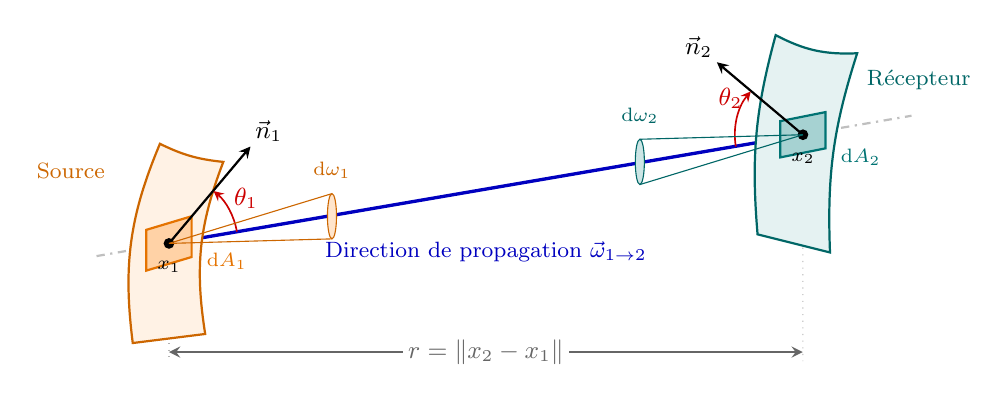
\begin{tikzpicture}[scale=1.15, >=stealth]
        % --- Définition des coordonnées centrales des facettes ---
        \coordinate (x1) at (0, 0);       % Centre de dA1 (Source)
        \coordinate (x2) at (7, 1.2);     % Centre de dA2 (Récepteur)

        % --- Axe optique direct (direction de propagation) ---
        % Angle de la ligne de visée x1 -> x2 : ~ 9.73°
        \draw[thick, dashdotted, gray!50] (-0.8, -0.14) -- (8.2, 1.41);
        \draw[very thick, ->, blue!75!black] (x1) -- (x2) 
            node[midway, below=15pt, font=\footnotesize] {Direction de propagation $\vec{\omega}_{1\to 2}$};

        % Cotation de la distance r
        \draw[<->, thick, gray!80!black] (0, -1.2) -- (7, -1.2)
            node[midway, fill=white, inner sep=2pt, font=\small] {$r = \|x_2 - x_1\|$};
        \draw[dotted, gray!60] (x1) -- (0, -1.3);
        \draw[dotted, gray!60] (x2) -- (7, -1.3);

        % ==============================================================
        % SURFACE 1 : Émetteur (Source dA1)
        % ==============================================================
        % Patch courbé source (centré en x1 = (0,0))
        \draw[thick, fill=orange!10, draw=orange!80!black] 
            (-0.4, -1.1) to[bend left=15] (-0.1, 1.1) 
                         to[bend right=10] (0.6, 0.9) 
                         to[bend right=15] (0.4, -1.0) -- cycle;
        \node[font=\footnotesize, orange!80!black, left] at (-0.6, 0.8) {Source};

        % Facette différentielle dA1 parfaitement centrée sur x1
        \draw[thick, fill=orange!35, draw=orange!90!black] 
            (-0.25, -0.3) -- (0.25, -0.15) -- (0.25, 0.3) -- (-0.25, 0.15) -- cycle;
        \filldraw[black] (x1) circle (1.5pt) node[below=3pt, font=\scriptsize] {$x_1$};
        \node[font=\scriptsize, orange!90!black, right=2pt] at (0.25, -0.2) {$\mathrm{d}A_1$};

        % Normale n1 (inclinée vers la direction de x2, angle ~ 50°)
        \coordinate (n1_end) at (0.9, 1.07);
        \draw[thick, ->, black] (x1) -- (n1_end) node[above right=-2pt, font=\small] {$\vec{n}_1$};

        % Arc pour l'angle theta 1 (entre axe 9.7° et n1 50°)
        \draw[->, semithick, red!80!black] (0.75, 0.13) arc (9.7:50:0.75);
        \node[red!80!black, font=\small] at (0.85, 0.5) {$\theta_1$};

        % Cône d'angle solide d\omega_1
        \coordinate (c1_top) at (1.8, 0.55);
        \coordinate (c1_bot) at (1.8, 0.05);
        \draw[thin, orange!80!black] (x1) -- (c1_top);
        \draw[thin, orange!80!black] (x1) -- (c1_bot);
        \draw[thin, fill=orange!20, draw=orange!80!black] (1.8, 0.3) ellipse (0.05 and 0.25);
        \node[font=\scriptsize, orange!80!black, above=2pt] at (1.8, 0.55) {$\mathrm{d}\omega_1$};

        % ==============================================================
        % SURFACE 2 : Récepteur (dA2)
        % ==============================================================
        % Patch courbé récepteur (centré en x2 = (7, 1.2))
        \draw[thick, fill=teal!10, draw=teal!80!black] 
            (6.5, 0.1) to[bend left=10] (6.7, 2.3) 
                       to[bend right=15] (7.6, 2.1) 
                       to[bend right=10] (7.3, -0.1) -- cycle;
        \node[font=\footnotesize, teal!80!black, right] at (7.6, 1.8) {Récepteur};

        % Facette différentielle dA2 parfaitement centrée sur x2
        \draw[thick, fill=teal!35, draw=teal!90!black] 
            (6.75, 0.95) -- (7.25, 1.05) -- (7.25, 1.45) -- (6.75, 1.35) -- cycle;
        \filldraw[black] (x2) circle (1.5pt) node[below=3pt, font=\scriptsize] {$x_2$};
        \node[font=\scriptsize, teal!90!black, right=2pt] at (7.25, 0.95) {$\mathrm{d}A_2$};

        % Normale n2 (inclinée vers x1, angle ~ 140°)
        \coordinate (n2_end) at (6.05, 2.0);
        \draw[thick, ->, black] (x2) -- (n2_end) node[above left=-2pt, font=\small] {$\vec{n}_2$};

        % Arc pour l'angle theta 2 (entre axe retour 189.7° et n2 140°)
        \draw[->, semithick, red!80!black] (6.26, 1.07) arc (189.7:140:0.75);
        \node[red!80!black, font=\small] at (6.2, 1.6) {$\theta_2$};

        % Cône d'angle solide d\omega_2
        \coordinate (c2_top) at (5.2, 1.15);
        \coordinate (c2_bot) at (5.2, 0.65);
        \draw[thin, teal!80!black] (x2) -- (c2_top);
        \draw[thin, teal!80!black] (x2) -- (c2_bot);
        \draw[thin, fill=teal!20, draw=teal!80!black] (5.2, 0.9) ellipse (0.05 and 0.25);
        \node[font=\scriptsize, teal!80!black, above=2pt] at (5.2, 1.15) {$\mathrm{d}\omega_2$};

    \end{tikzpicture}
    \caption{Transport radiatif différentiel entre deux éléments de surface orientés $\mathrm{d}A_1$ et $\mathrm{d}A_2$ séparés par une distance $r$.}
    \label{fig:transfert_radiatif_surfaces}
\end{figure}